\chapter{Datasets} % Main appendix title

\label{AppendixD} % For referencing this appendix elsewhere, use \ref{AppendixX}

\section{Audi}

The  Audi Autonomous Driving Dataset (A2D2)
authors (\cite{geyer2020a2d2}) are motivated by the fact that research in machine learning, mobile robotics and autonomous driving is accelerated by the availability of high quality annotated data. This statement can be verified by the advances in image classification with deep neural networks since \cite{IMAGENET} became available.  
The A2D2 data was acquired with a human-driven Audi Q7 e-tron equipped with six cameras (front left, front center, front right, back left, back center, back right) and five LiDAR sensors. The authors claim this resulted in  360$^{\circ}$ camera and LiDAR coverage. Additionally, several bus data signals from the vehicle were recorded such as velocity, acceleration and steering wheel angle. 
The total size is 2.3TB. Our datasets of interest are the  Though, since we are interested in image and steering angle only, our data can be narrowed to 
\begin{verbatim}
    https://aev-autonomous-driving-dataset.s3.eu-central-1.amazonaws.com/README-SensorFusion.txt
    
- steering_angle_calculated
- steering_angle_calculated_sign

- 'cam_front_center'
\end{verbatim}

The dataset total size is approximately 2.3TB and provides (...) TBC following https://www.a2d2.audi/a2d2/en/download.html

This was supplied for three cities: Gaimersheim, Ingolstadt and Munich. To perform initial investigations we chose data from Munich and downloaded the "Camera - Front Center" images, constituting 27451 images 3.2MB in size each and dimension 1920x1208 pixels, total size on disk is about 92GB. We also downloaded the 176MB "Bus Signals" file. The image naming convention uses a timestamp in the format:
\begin{verbatim}
20190401145936_camera_frontcenter_000017970.png
\end{verbatim}
The "Bus Signals" file is JSON encoded and provides several signals such as acceleration, angular velocity and vehicle speed. Our signals of interest are the steering angle calculated and steering angle sign. In the bus signals file (20190401121727\_bus\_signals.json) we parsed our values of interest e.g.
\begin{verbatim}
(...)
    "steering_angle_calculated": {
        "unit": "Unit_DegreOfArc",
        "values": [
            [
                1554115464698116,
                2.4
            ],
(...)
\end{verbatim}
where the unit is degree of arc and the values are inferred to be a timestamp when the measurement was acquired and the angle (1554115464698116 and 2.4 respectively, in the example shown).
and found 91968 entries for each of the steering angle and sign. This is over 3 times the amount of corresponding images. Since there was no obvious key to match the steering angle and sign with a corresponding image, we wrote to the supplied enquiry email address aevdrivingdataset@audi.de with regard to this problem and receiving no reply, abandoned the dataset deeming it unusable for our purposes.  
Note: we did try converting the integer into a date using python, which resulted in an error:
\begin{verbatim}
import datetime
audi_timestamp = 1554115464698116
date = datetime.datetime.fromtimestamp(audi_timestamp / 1e3)
print(date)
# ValueError: year 51217 is out of range    
\end{verbatim}

TODO ADD BINS
\begin{figure}[ht]
 \centering 
 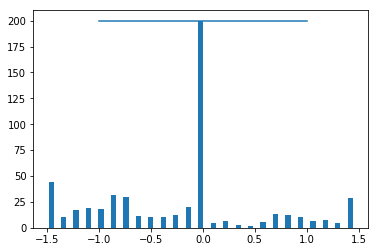
\includegraphics[scale=1]{Figures/bins.png}
 \caption{Diagram showing bins centered around zero degrees, meaning most of time car is driving straight. Binning diagrams for all datasets can be found in appendix B}
 \label{fig:bins-placeholder}
\end{figure}

%% TODO add correspondence with Mentar

\section{Udacity}

1. Link trail - medium (Indian guy) -> medium (Chinese guy)-> github (Japanese guy)  
  
2. Udacity data  
Data is available for download in torrent file format (\cite{torrentCite}) and consist of Robot Operating System (ROS) rosbag compressed files.

\begin{verbatim}
https://github.com/udacity/self-driving-car/tree/master/datasets
\end{verbatim}
3. Rosbag

\section{utbm}
More stuff from german uni?
\begin{verbatim}
https://epan-utbm.github.io/utbm_robocar_dataset/
\end{verbatim}

TODO ADD BINS
\begin{figure}[ht]
 \centering 
 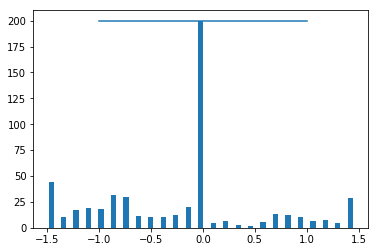
\includegraphics[scale=1]{Figures/bins.png}
 \caption{Diagram showing bins centered around zero degrees, meaning most of time car is driving straight. Binning diagrams for all datasets can be found in appendix B}
 \label{fig:bins-placeholder}
\end{figure}

\section{Training Log}

\begin{verbatim}
Run ID  Data       Network Acc. Error Saved Best Model 
3       log_sample NVIDIA1
\end{verbatim}

Run ID  Data    Network Training    Acc Error   Saved Best Model    Saved History
%1       Udacity 1       SGD Adam    .95 .06     model_01            history_01

\subsection{Run 3}

This model has a single output, steering angle, and produced very low accuracy.
Notes:
\begin{verbatim}
commit 423b5b783565b60e72f970485d9b3aa9887f5453
training time
dataset: sample_data
\end{verbatim}

\subsection{Run 4 - }

% Naoki's model not doing well, sanity check with one output
Also not doing well
Next run, 2 outputs (steering and throttle)

\subsection{Run 5 - 20201102081239} 

\begin{verbatim}
commit 076e8b32664738df6af9e14d75355504eb2a94b4
Much better results with two outputs. 
cat ../dataset/unity/log_sample/logs_Mon_Jul_13_08_29_01_2020/record_11659.json
Both are floats - steering angle and throttle
loss: 0.0105 - acc: 0.8502 - val_loss: 0.0111 - val_acc: 0.8617

dataset: sample_data
model: nvidia1
outputs: 2
\end{verbatim}

\subsection{Run 5 - 20201102090041\_nvidia2}
\begin{verbatim}
commit 42dabb6321ad25f667c8663b63412c88c96b3b38
model: nvidia2
outputs: 2
dataset: log_sample (size: 12k)
$ python train.py --model=nvidia2 --outdir=../trained_models
loss: 0.0108 - acc: 0.8483 - val_loss: 0.0117 - val_acc: 0.8495
\end{verbatim}

\subsection{Run 6 - 20201102094552\_nvidia1}
\begin{verbatim}
commit ec9d081b85f7386365428a73896b1d09be7ba917
model: nvidia1
outputs: 2
dataset: log2 (280727)
command
$ train.py --model=nvidia1 --outdir=../trained_models
loss: 0.0077 - acc: 0.8726 - val_loss: 0.0077 - val_acc: 0.8732
\end{verbatim}

\subsection{Run 7 - 20201102090041_nvidia2.h5}
\begin{verbatim}
commit 1da10b6745f583e180d5b9c5ba4874847ba8610c
model: nvidia2
outputs: 2
dataset: log2
command
$ train.py --model=nvidia2 --outdir=../trained_models
\end{verbatim}

\subsection{Run 8 - 20201102134802_nvidia2.h5}
\begin{verbatim}
commit 6960f2f5fb50b565c0dfd6c8fe3ac1d283192e69
model nvidia2
outputs 2
dataset log2
command:
train.py --model=nvidia2 --outdir=../trained_models
\end{verbatim}


\subsection{Run 9 - 20201102210514_nvidia2.h5}
\begin{verbatim}
Running nvidia2 with augmentation
commit 
model nvidia2
outputs
dataset
command:
\end{verbatim}

\subsection{Run 10 - }
\begin{verbatim}
Run NVIDIA1 WITHOUT augmentation
commit 
model
outputs
dataset
command:
\end{verbatim}

\subsection{Run X - }
\begin{verbatim}
commit 
model
outputs
dataset
command:
\end{verbatim}





